En esta sección mostraremos el Diagrama de interrelación de documentos(DID) creado a partir del DER mostrado en la sección
anterior.

\begin{figure}[H]
  \centering
    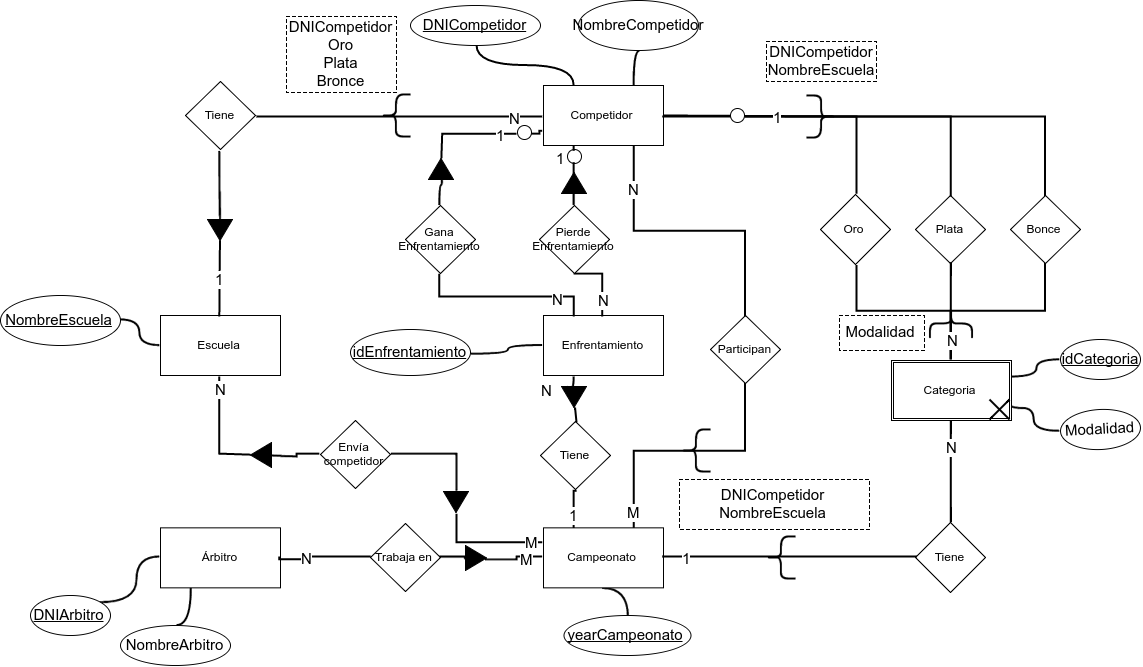
\includegraphics[scale=0.4]{imagenes/DID.png}
  \caption{Diagrama entidad relación}
\end{figure}

A continuación mostraremos la forma en la que se resolvieron las consultas pedidas y justificaremos como las decisiones
tomadas las optimizan.

\subsection{Consultas}
\begin{enumerate}
\item Se nos pide la cantidad de enfrentamientos ganados por competidor para un campeonato dado. Se nos da como parámetro
el año del campeonato. Para resolver la consulta, recorremos todos los enfrentamientos. Contamos la cantidad de
enfrentamientos ganados para cada competidor que coincidan con el año del campeonato. Esto lo podemos realizar de forma óptima
ya que el enfrentamiento referencia a campeonato, por lo tanto tiene el año del campeonato. Además referencia al ganador y al
perdedor, por lo tanto puede usarlos para contar la cantidad de victorias por cada competidor.

\item La cantidad de medallas por nombre de escuela en toda la historia. Itero en el documento Escuela y por cada una
recorro la ListaCompetidores. Para cada competidor, realizo la suma de las medallas de los tres tipos(oro
, plata y bronce). La suma de las medallas de cada competidor en las escuelas se beneficia del hecho de que cada escuela
posee la ListaCompetidores gracias a que se tomo la decisión embebido parcialmente a los competidores en el documento
Escuela. La lista de competidores contiene la cantidad de medallas de cada uno de los tres tipos que cada competidor obtuvo
históricamente. Solo hace falta sumar los tres tipos para obtener el histórico de medallas del competidor.

\item Para cada escuela, el campeonato donde ganó más medalla. La consulta se divide en dos partes. La primer parte consiste
en recorrer todos los campeonatos y guardarme las categorías que están en ListaCategorias, utilizando para esto el año del
campeonato. En la segunda parte recorro todas las entradas en el documento Escuela. Por cada una de estas, utilizo las
categorías guardadas en el paso anterior. Recorro todas las categorías y, por cada una, cuento la cantidad de ganadores de
medallas que pertenecen a la escuela. Esta consulta está optimizada usando que Campeonato tiene embebido a Categoria, con lo
cual podemos adquirir de cada campeonato los ganadores de medallas de los tres tipos. Además Categoria tiene embebido parcialmente
a Competidor por el atributo NombreEscuela, con lo cual podemos usar este dato para identificar a la escuela que pertenece cada
medalla. Por último, el documento Escuela tiene una referencia a Campeonato. Esto significa que Escuela tiene los yearCampeonato
de todos en los que mando competidores. En el primer paso habíamos guardado las categorías por el año del campeonato y ,
gracias a esta referencia de Campeonato en Escuela, podemos acceder a las categorías. Por consiguiente, tenemos acceso a la
información sobre los ganadores de medallas. Dado que necesitamos la información de las medallas, la consulta pareciera que
se puede resolver tanto usando el documento Campeonato como el documento Competidor. Sin embargo, esto no es cierto ya que
a través de competidor no podemos diferenciar los campeonatos en los cuales cada uno gano las medallas. Por eso necesitamos recorrer
los campeonatos para obtener las categorías y después ver en cuales los competidores de cada escuela resultaron vencedores.

\item Los árbitros que participaron en al menos 4 campeonatos. La consulta se realiza recorriendo los documentos
de Árbitro contando los Campeonatos usando ListaCampeonatos. Finalmente nos quedamos con los árbitros donde la ListaCampeonatos
tiene, al menos, 4 campeonatos distintos. Para cada árbitro, el proceso se resume en contar los campeonatos en la lista.
Podemos realizar esto gracias a ListaCampeonatos, la cual obtenemos gracias a que el documento Arbitro posee referencias
al documento Campeonato.

\item Las escuelas que han presentado el mayor número de competidores en cada campeonato. Recorro el conjunto de documentos
Campeonato y para cada uno recorro su ListaCompetidores y cuento, por cada NombreEscuela, la cantidad de competidores.
La consulta es optimizada debido a que los Campeonatos tiene embebido parcialmente a Competidor por el atributo
NombreEscuela. Con lo cual, no se necesita acceder a otro documento que no sean todas las entradas de Campeonatos.
Esto último es necesario ya que necesitamos información de todos los Campeonatos para encontrar a las escuelas en las
que más competidores participaron.

\item Obtener los competidores que más medallas obtuvieron por modalidad. Por cada entrada de el documento Campeonato,
cuento las medallas de cada tipo que coinciden con cada modalidad. Después me quedo con el DNICompetidor a los cuales
son ganadores de más medallas de cada tipo. Esta consulta se beneficia de que el CompCampeonatoetidor tiene embebido
el documento Categoría. Por lo tanto, no es necesario acceder a ningún otro documento que no sea Campeonato. Desde el embebido
 de Categoria obtengo los DNS's de los competidores que resultaron ganadores.

\end{enumerate}
